\chapter{How Eyes Work}

Dr. Craig Blackwell has made a great video on the mechanics of the
eye. You should watch it: \url{https://youtu.be/Z8asc2SfFHM}

Mechanically, your eye works a lot like a camera.  The eye is a sphere
with two lenses on the front: The outer lens is called the \newterm{cornea}, and the
second lens is just called ``the lens.''

Between the two lenses is an aperture that opens wide when there is
very little light, and closes very small when there is bright light.
The opening is called the \newterm{pupil} and the tissue that forms
the pupil is called the \newterm{iris}. When people talk of the color
of your eyes, they are talking about the color of your iris. The
blackness at the center of your iris is your pupil.

There are two types of photoreceptor cells in your retina: rods and
cones. The rods are more sensitive; in very dark conditions, most of
our vision is provided by the rods. The cones are used when there is
plenty of light, and they let us see colors.

The white part around the outside of the eyeball? That is called the
\newterm{sclera}.

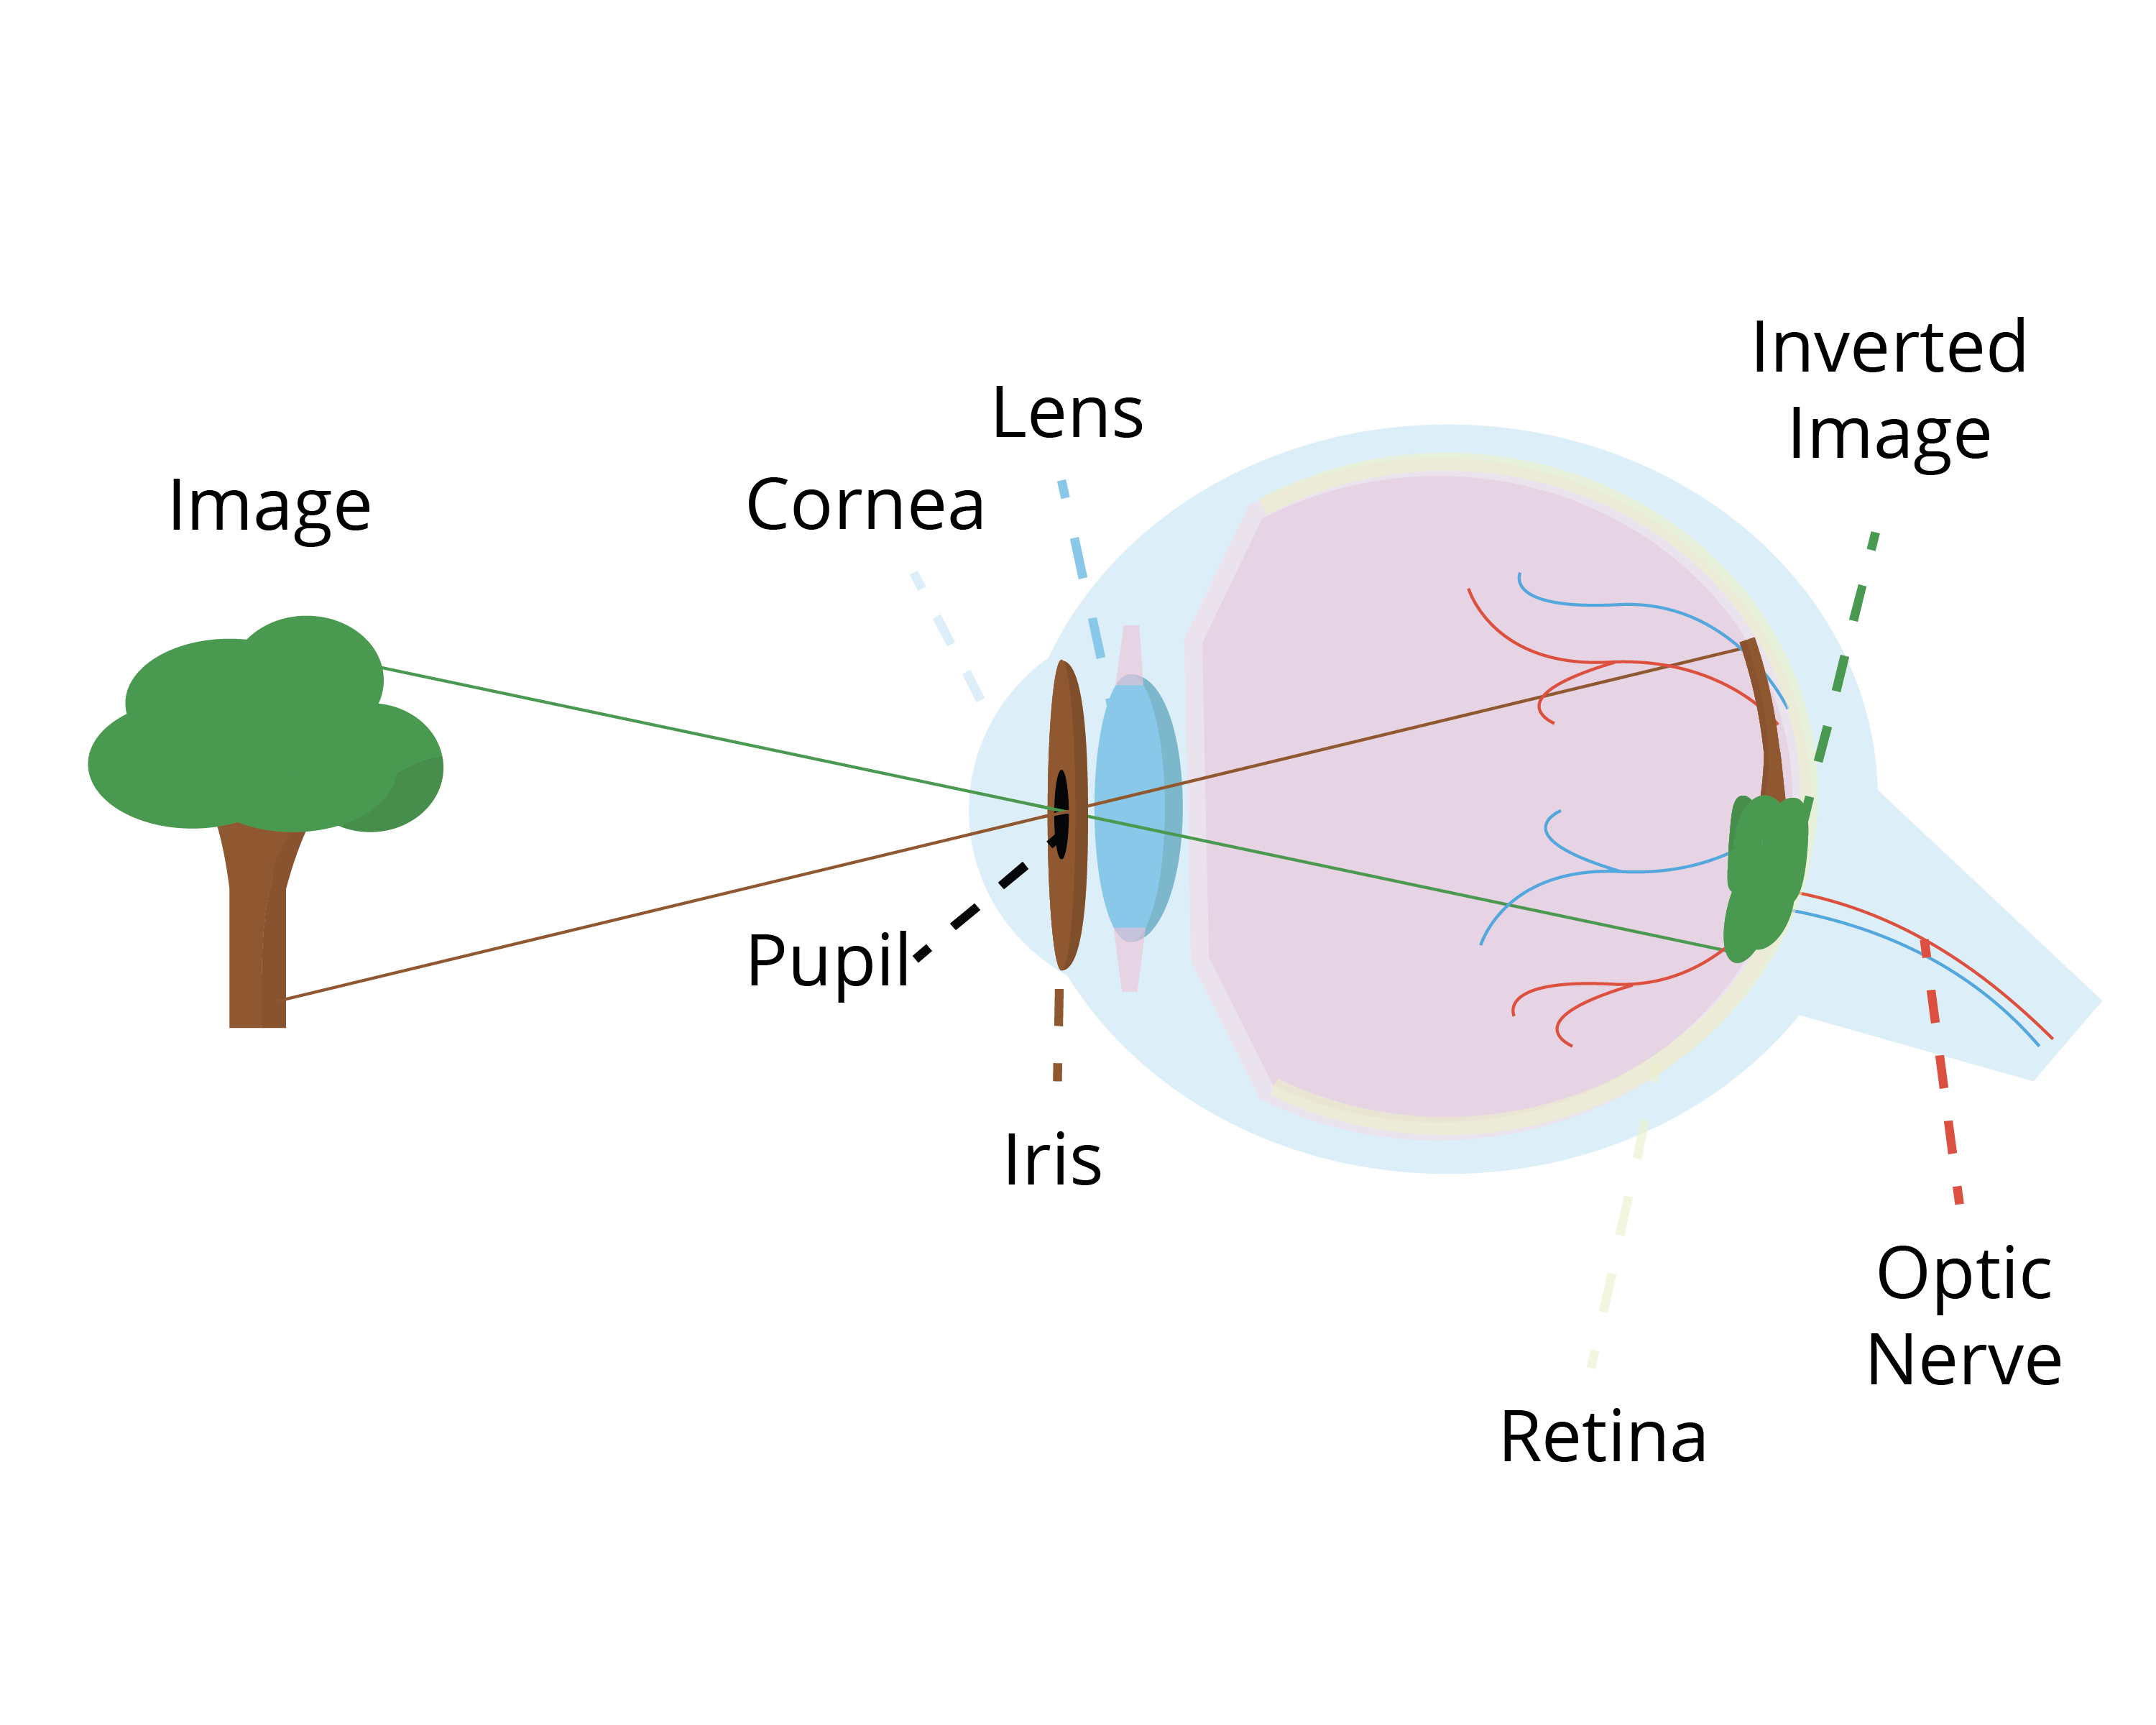
\includegraphics[width=0.8\textwidth]{eyeDiagram.png}

The walls of the eye are lined inside with the \newterm{retina}, which has
 sensors that pick up the light and send impulses down the optic
nerve to your brain.

Just like a camera, the images are flipped when they get projected on
the back of the eye.

\section{Eye problems}

Now that you know the mechanics of the eye, let's enumerate a few
things that commonly go wrong with the eye.

\subsection{Glaucoma}

The space between your cornea and lens is filled with a fluid called
\newterm{aqueous humor}. To feed the cells of the cornea and lens,
the aqueous humor carries oxygen and nutrients like blood would, but
it is transparent so you can see. Aqueous humor is constantly being
pumped into and out of that chamber.  If aqueous humor has trouble
exiting, the pressure builds up and can damage the eye. This is known
as \newterm{glaucoma}.

\subsection{Cataracts}

The lens should be clear. As a person ages (and it can be accelerated
by diabetes, too much exposure to sunlight, smoking, obesity, and high
blood pressure), the proteins in the lens break down and clump
together, becoming opaque. From the outside, the eye will look
cloudy. This is called a \newterm{cataract}, and it makes it difficult
for the person to see.

The problem can be corrected: The person's cloudy lens is removed and
replaced with a clear, manufactured lens.
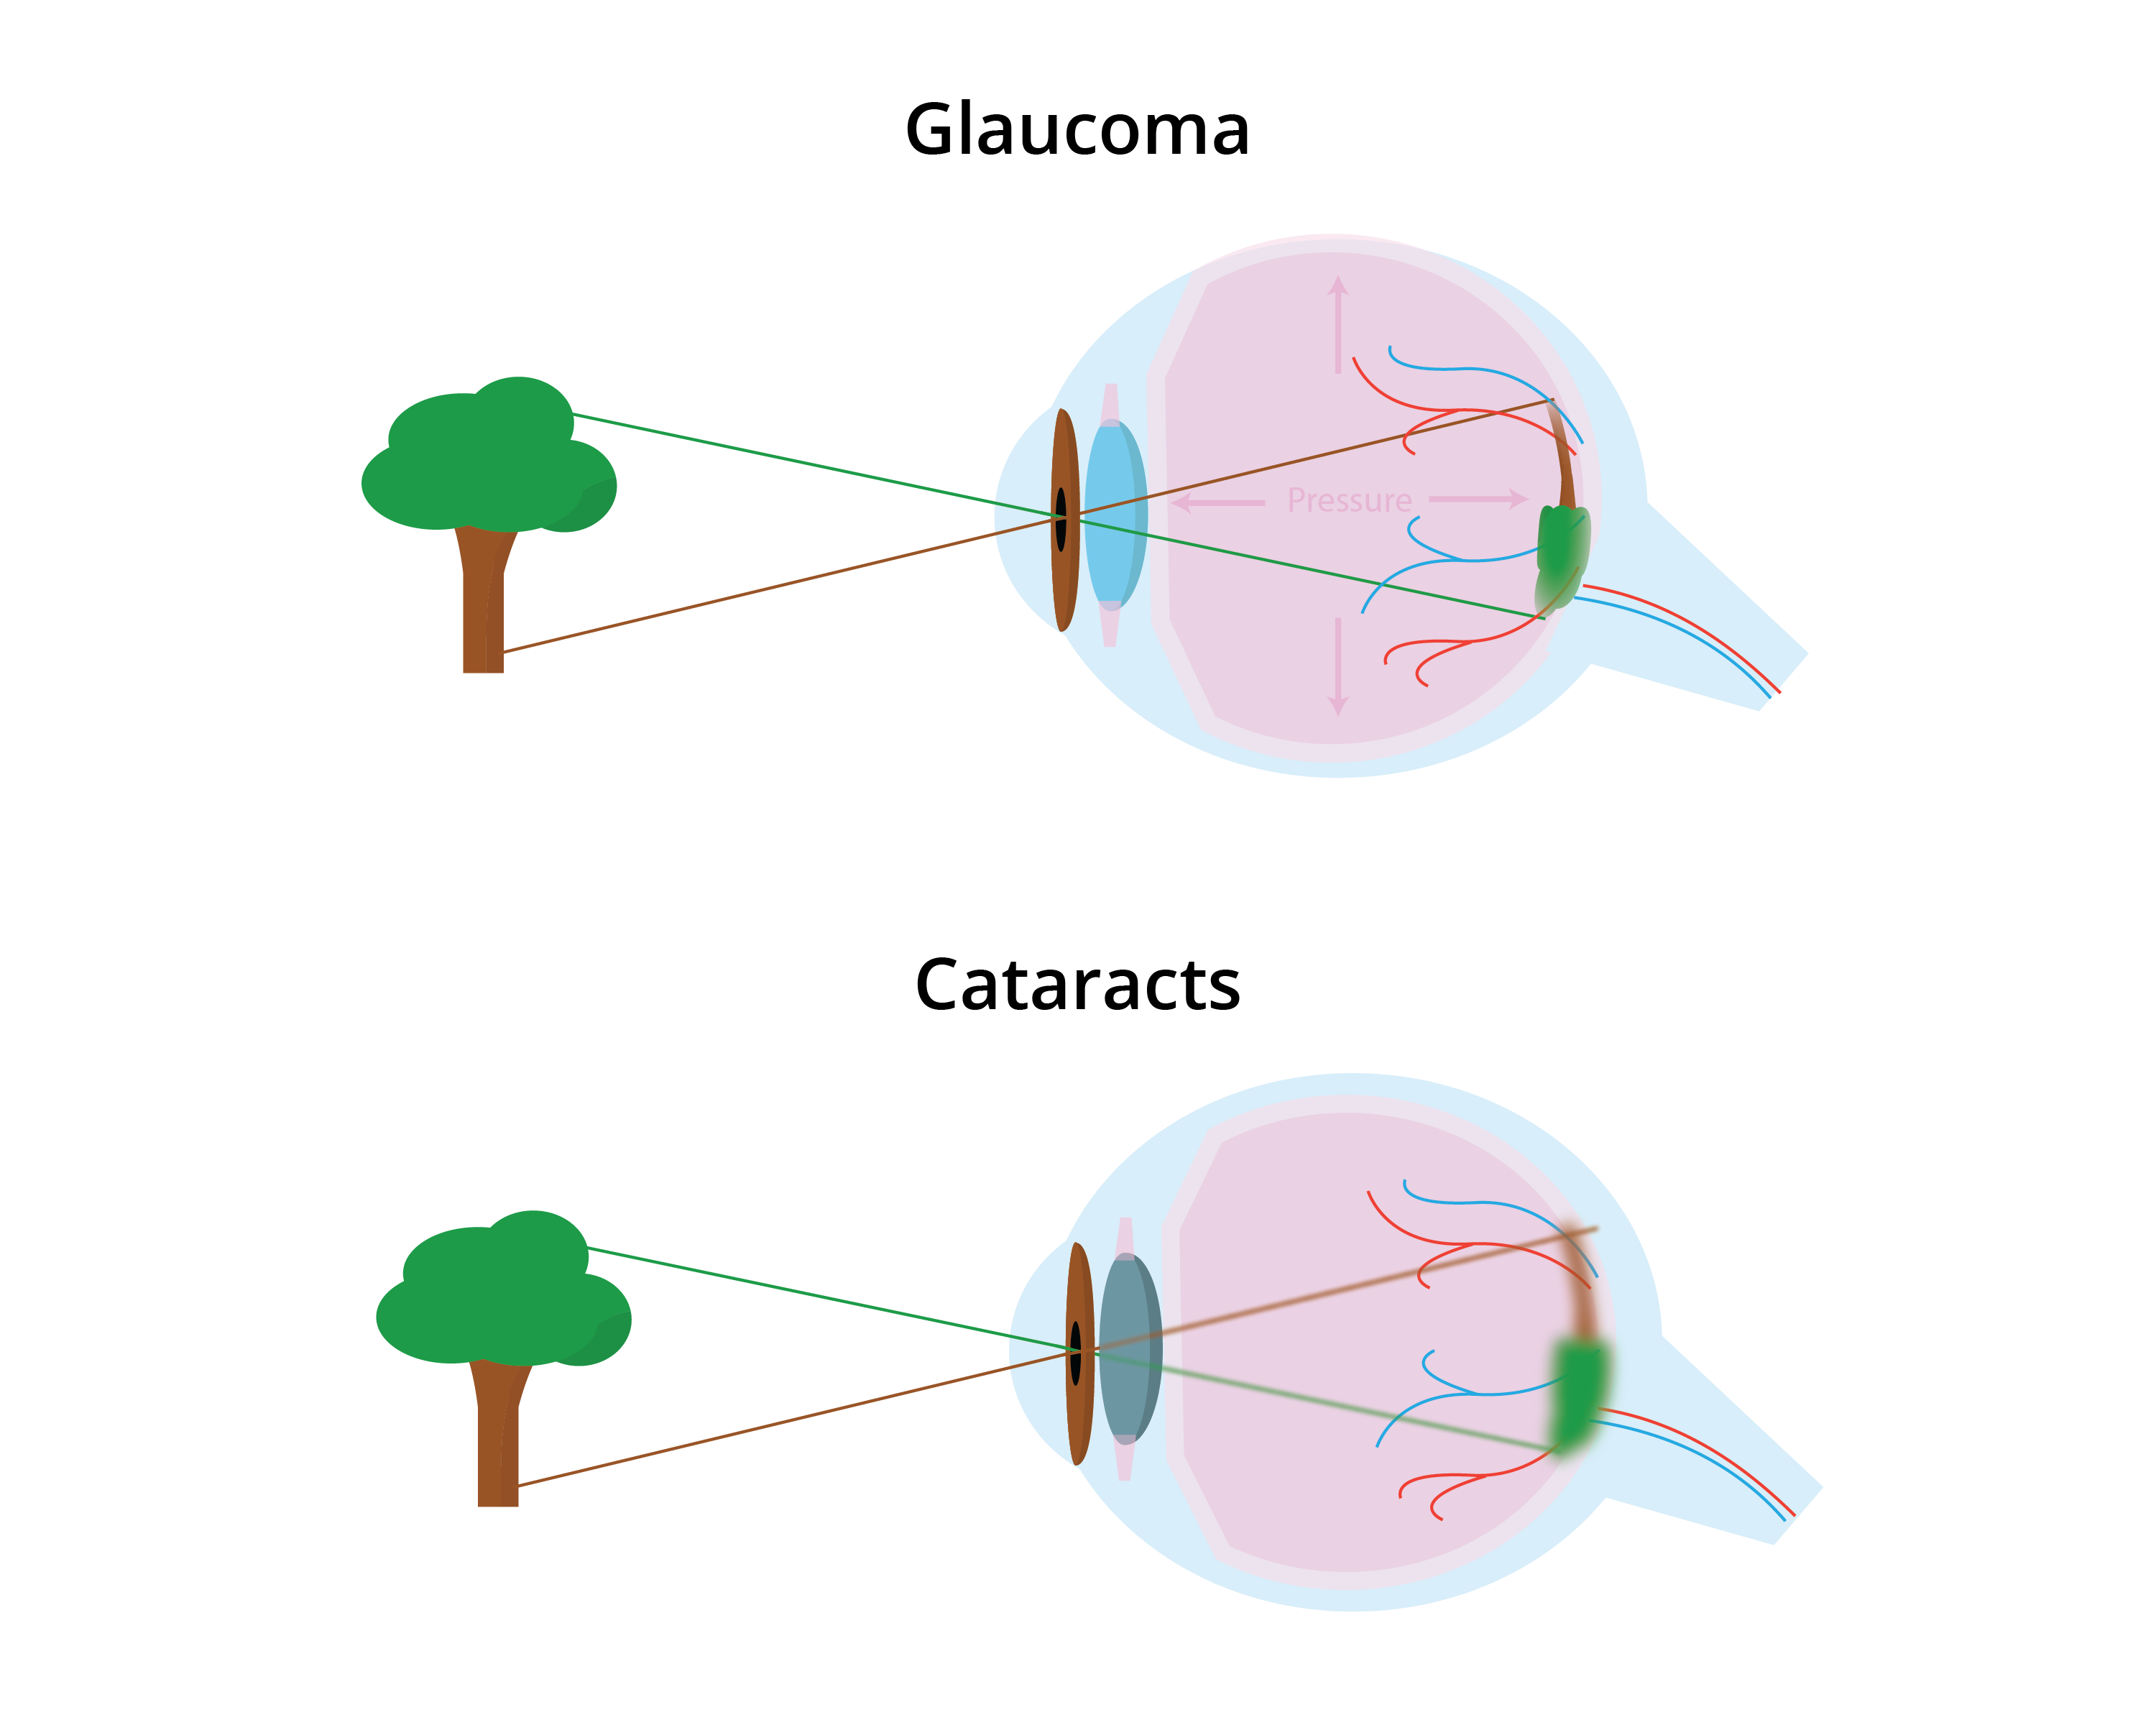
\includegraphics[width=0.8\textwidth]{cataractGlaucoma.png}

\subsection{Nearsightedness, farsightedness, and astigmatism}

If you are in a dark room and a tiny LED is turned on, the photons
from that LED can pass through your cornea in many different places.
If your eye is focusing on that light correctly, all the photons
should meet up at the same place on the retina.

FIXME: Diagram here

If the lenses are bending the light too much, the photons meet up before they hit the
retina and get smeared a bit across the retina. To the person, the LED
would appear blurry. The eye is said to be \newterm{nearsighted} or
\newterm{myopic}.

If the lenses are not bending it enough, the photons would meet up
behind the retina.  Once again, they get smeared a bit across the
retina and the LED looks blurry to the person. The eye is said to be
\newterm{farsighted} or \newterm{hyperoptic}.

Your lenses are supposed to bend the photons the same amount
vertically and horizontally. If one dimension is focused, but the
other is myopic or hyperoptic, the eye is said to have \newterm{astigmatism}.

Myopia, hyperoptia, and astigmatism can be corrected with glasses or contact
lenses. Doctors can also do surgical corrections, usually by changing
the shape of the cornea.
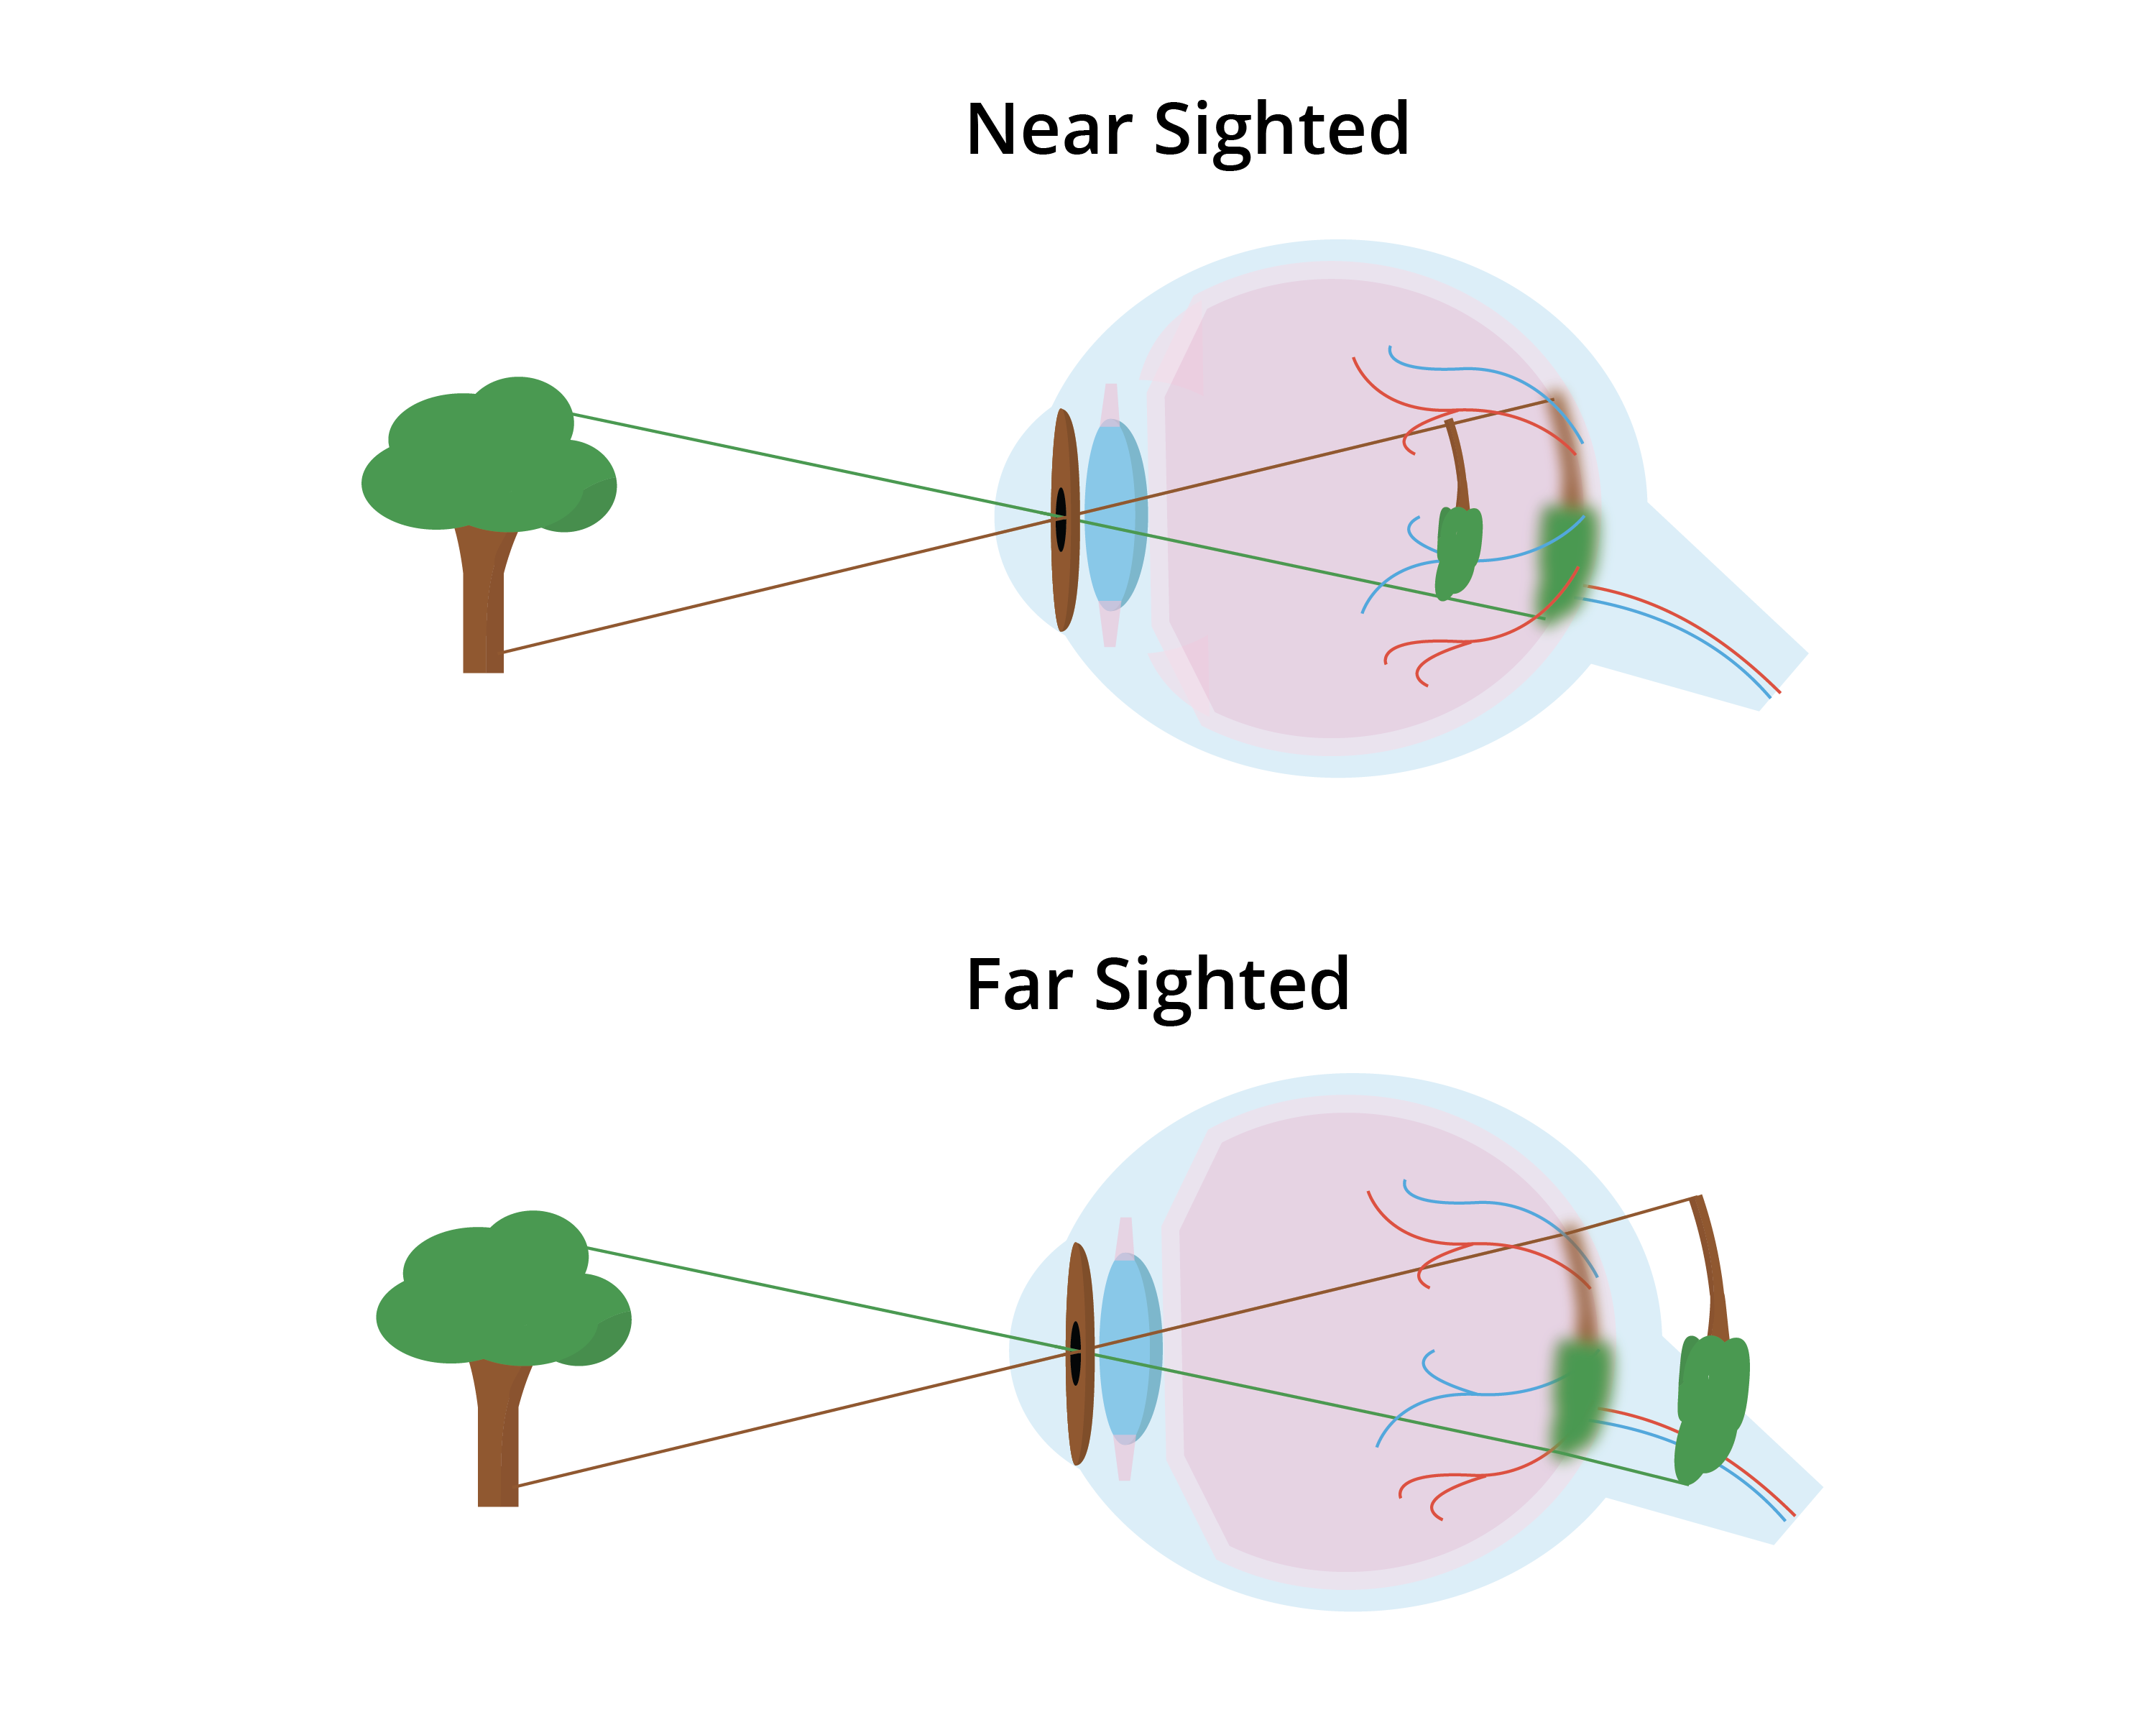
\includegraphics[width=0.75\textwidth]{nearfarSight.png}

\section{Seeing colors}

TED-Ed has made a good video on how we see color. Watch it here: \url{https://youtu.be/l8_fZPHasdo}

When a rainbow forms, you are seeing different wavelengths separating from each other. In the rainbow:
\begin{itemize}
\item Red is about 650 nm.
\item Orange is about 600 nm.
\item Yellow is about 580 nm.
\item Green is about 550 nm.
\item Cyan is about 500 nm.
\item Blue is about 450 nm.
\item Violet is about 400 nm.
\end{itemize}

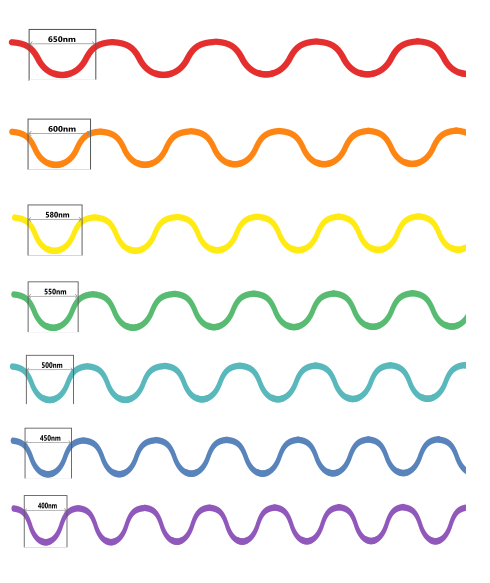
\includegraphics[width=0.75\textwidth]{Color_Waves.png}

If you shine a light with a wavelength of 580 nm on a white piece of
paper, you will see yellow.

However, if you shine two lights with wavelengths of 650 nm (red) and
550 nm (green), you will also see yellow.

Why? Our ears can hear two different frequencies at the same time.
Why can't our eyes see two colors in the same place?

As mentioned above, the cone photoreceptors in our eyes let us see
colors. There are three kinds of cones:
\begin{itemize}
  \item Blue: Cones that are most sensitive to frequencies near 450nm.
  \item Green: Cones that are most sensitive to frequencies near 550nm.
  \item Red: Cones that let us see the frequencies up to about 700nm.
\end{itemize}

When a wavelength of 580 nm hits your retina, it excites the red
and green receptors, and your brain interprets that mix as yellow.

Similarly, when light that contains both 650 nm and 550 nm waves hits
your retina, it excites the red and green receptors, and your brain
interprets that mix as yellow.

You can't tell the difference!

Now we know why the sensors on the camera are RGB. The camera is
recording the scene as closely as necessary to fool your eye.

A TV or a color computer monitor only has three colors of pixels: red,
green, and blue.  By controlling the mix of them, it creates the
sensation of thousands of colors to your eye.

\section{Pigments}

A color printer works oppositely: Instead of radiating
colors, it puts pigments on the paper that absorb certain frequencies.
A pigment that absorbs only frequencies near 650 nm (red) will appear
to your eye as cyan. This makes sense because the sensation of cyan is
created when your blue and green receptors are activated.

Thus, pigment colors come in:
\begin{itemize}
\item Cyan: absorbs frequencies around red
\item Magenta: absorbs freqencies around green
\item Yellow: absorbs frequencies around blue
\end{itemize}

If you buy ink for a color printer, you know there is typically a
fourth ink: black. If you put cyan, magenta, and yellow pigments on
paper, the mix won't absorb all the visible spectrum in a consistent
manner, and our eyes are pretty sensitive to that, so we would see
brown. So we add black ink to get pretty grays and blacks.

We call this approach to color CMYK (as opposed to RGB). If an artist
is creating an image to be viewed on a screen, they will typically
make an RGB image.  If they are creating an image to be printed using
pigments, they typically create a CMYK image. (Most of us don't care
so much -- we just let the computer do conversions between the two
color spaces for us.)

